\documentclass[9pt,onecolumn,oneside,lineno]{pnas-new}
%\documentclass[12pt,twocolumn]{article}
%\documentclass[twocolumn]{biophys}
%\usepackage{amssymb,amsfonts,amsthm,bm}
%\usepackage[round,numbers,sort&compress]{natbib}
%\usepackage[ansinew]{inputenc}
%\gridframe{N}
%\templatetype{pnassupportinginfo}
%\title{PNAS Supporting Information Template}
%\author{LeadAuthor et al.}
\newcommand{\fivering}{interfacial band~}
\newcommand{\fiveringnos}{interfacial band}
\newcommand{\triad}{pore oscillator~}
\newcommand{\triadns}{pore oscillator~}
\usepackage{amssymb,amsfonts,amsthm,bm}
\usepackage{adjustbox}
\usepackage[round,numbers,sort&compress]{natbib}
\usepackage{graphicx}
\usepackage{amssymb}
\usepackage{fixltx2e}
\usepackage{graphicx}
\usepackage{wrapfig, blindtext}
\usepackage{setspace}  
\usepackage{texshade}
%\usepackage{caption}
%\usepackage{subcaption}
%\usepackage{subfig}
%\usepackage[ansinew]{inputenc}

\begin{document}
%\maketitle
\newcommand{\grace}[1]{\textcolor{blue}{#1}}
%\section*{Supporting Information (SI)}
\newcommand{\GABAA}{GABA\textsubscript{A}R\xspace}
\newcommand{\avgr}{\bar{r}}
\newcommand{\varr}{\delta r^{2}}
\newcommand{\plgics}{pLGICs}
\newcommand{\nachr}{nAChR}
\renewcommand{\thefigure}{S\arabic{figure}}
\newcommand{\WT}{WT\xspace}
\newcommand{\MT}{K289M\xspace}
\newcommand{\RMSD}{RMSD\textsubscript{symm}\xspace}
\newcommand{\WTs}{WT systems\xspace}
\newcommand{\MTs}{K289M systems\xspace}
\newcommand{\RMSDs}{RMSDs\textsubscript{symm}\xspace}
\setcounter{figure}{0}
%\begin{figure}
%\begin{center}
%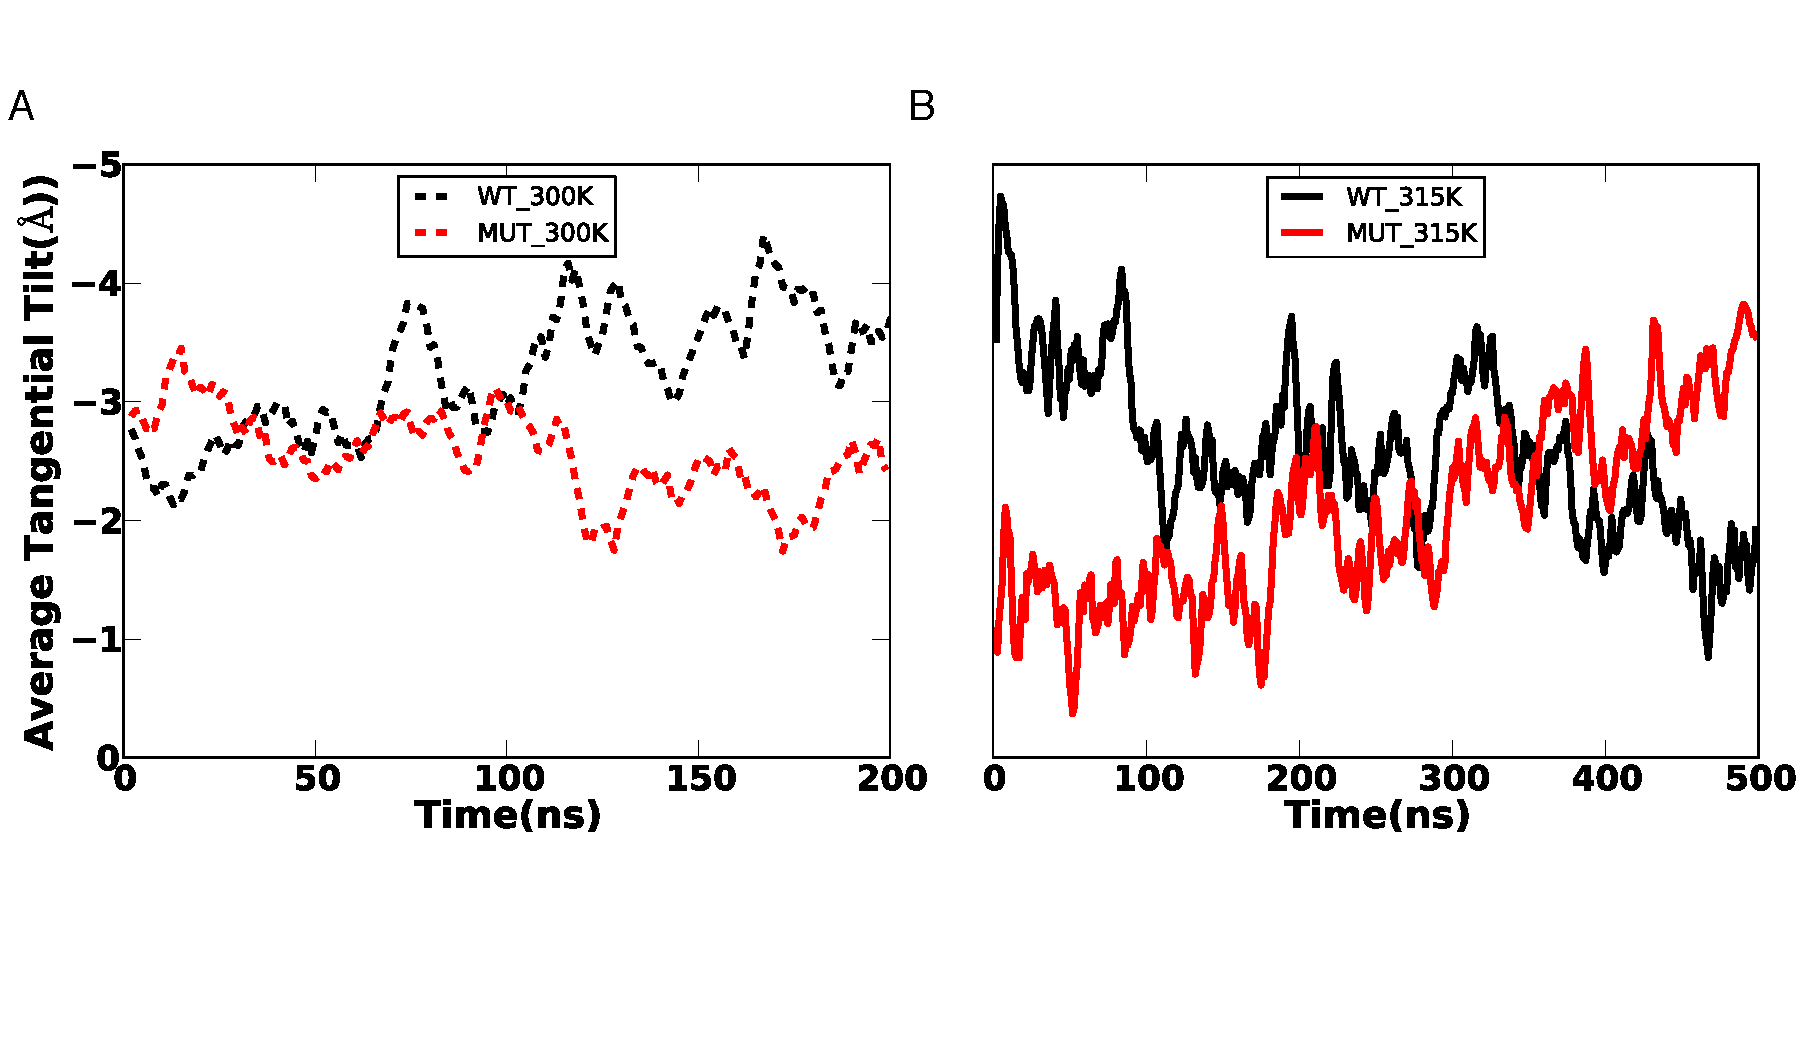
\includegraphics[width = 1\textwidth]{figures/Sup-tangential_tilt.pdf}
%\end{center}
%\caption{Average Tangential Tilt of the M2 helices (A) at 300K and (B). at 315K.}
%\label{fig:avgTilt}
%\end{figure}

\section*{Supporting Methods}

%A high resolution structure of a \GABAA was not available until the publication of the 3\AA~resolution structure for a \(\beta\)\textsubscript{3} homopentamer.\cite{Miller2014}  In the transmembrane domain, homology between \GABAA $\alpha$ or $\gamma$ to \GABAA $\beta$  is not significantly improved relative to homology between \GABAA $\alpha$/$\gamma$ subunits and GluCl$\alpha$, 
%%GB: need numbers
%and as a result homology models of $\alpha\beta\gamma$\GABAA built on the \GABAA $\beta_3$ homopentamer are not expected to be significantly improved relative to those based on GluCl.
The systems were solvated using the SOLVATE plugin in VMD\cite{Humphrey1996a} and neutralizing ions were added to bring the system to a 0.15M salt concentration using the AUTOIONIZE plugin. The final system contained about 160,000 atoms. MUTATE plugin was used to introduce the K289M mutation in the $\gamma$ subunit of \GABAA receptor.

All bonds to the hydrogen atoms were constrained using the SHAKE/RATTLE algorithm. A multiple time-step rRESPA method was used, and controlled with a high frequency time-step of 2fs and low frequency time-step of 4fs. 
All the systems were energy minimized for 10000 steps, then simulated for 5 ns with restraints of 1 kcal/mol/\AA\ applied to the C\textsubscript{\(\alpha\)} atoms of the protein. Restraints were then removed and 495 ns of nearly unrestrained simulation was carried out in all four systems at low temperature. During this period of the simulation, only harmonic restraints (force constant 0.4 kcal/mol/\AA) between the intracellular ends of the M3 and M4 helices were used, to mimic the effects of the intracellular domain and prevent separation of the M4 helix from the rest of the bundle.

\subsection*{Long-range electrostatics}

The simulations here used the prescribed cutoff value of 12 $\AA$ for the CHARMM forcefield, with a switching function past 10$\AA$, combined with PME and a grid size of about 1\AA.   The distances between charged residues in the \fivering are similar to this cutoff distance, and it is not uncommon to use cutoffs less than 10\AA (as in \cite{Lev2017}).  This may cause a significant accumulated error in simulations of any proteins with repeated interactions near the cutoff/switching distance, not just pLGICs. In pLGICs, it can reduce the energetic cost of shrinking the \fiveringnos, leading to an increased likelihood of closed states even in \WT systems. By recalculating energies using direct Coulomb electrostatics just for \fivering and \triad residues, from a trajectory generated using PME, we found PME reduced the energetic difference between elongated and regular conformations by about 5~kcal/mol. 

\subsection*{SMD Simulations} Steered Molecular Dynamics (SMD) simulations \cite{Isralewitz2001,Park2004}
were used to obtain favorable positions of the ion at different positions along the channel, for later use in Adaptive Biasing Force (ABF) calculations. The chloride ion was pulled along the pore of the channel  at a constant velocity of 10\AA\//ns. The force required to pull at constant velocity is also calculated, and can, in principle, be used to calculate a potential of mean force (PMF) using Jarzynski's equation \cite{Jarzynski1997,Jarzynski1997a}, but in practice it is challenging to achieve a sufficiently slow pulling speed. 

\subsection*{ABF Simulations} Adaptive biasing force calculations (ABF)\cite{Henin2004,Darve2008,Pohorille2010,Comer2014}  were used to measure the potential of mean force (PMF)  of a chloride ion translocating the \GABAA ion channel at 315K, for both the \WT\ and \MT\ channels. ABF was performed using the Collective Variables module\cite{Fiorin2013} of NAMD2.9.  The pore axis was divided into 23 bins of each 5\AA\ length.

Initial coordinates for the ion were obtained from SMD simulations (as described in SI). One thousand samples were collected in each bin prior to the application of ABF  to avoid undesired non-equilibrium effects on the dynamics. Fifteen ns of trajectory were generated in most bins, while bins near the primary barrier in the pore contained 25 ns. 

\subsection*{Pore Analysis} Measurement and analysis of the pore radii has been carried out using the HOLE software \cite{Smart1996} and TCL scripting through VMD\cite{Humphrey1996a}. Python scripts have been used to analyze and visualize the hydration of the pore throughout the simulation. 

\subsection*{Poisson-Boltzmann Calculations} The Poisson-Boltzmann (PB) profile for conduction of both a Na+ and Cl- through the ion channel was calculated using APBSmem\cite{Callenberg2010}. The pre-generated PQR format of the proteins using PDB2PQR\cite{Dolinsky2007} tool was used as the input for the electrostatic potential calculations.

These calculations were performed for initial non-equilibrated structures of the protein, as well as for conformations extracted from the last 50 ns of both the 300K and 315K MD simulations (for Cl-). 

\subsection*{Graphs and images}
All plots were calculated and drawn using Python and Tcl scripts.In Figure 2 and the similar supplementary figures S5-S11, the series of curves depicting the pore-opening events were further smoothened using a digital filter(Butterworth) with a order of the filter value, 2, and a critical frequency value, 0.02,  as implemented in the SciPy python module. The time derivative of the minimum pore radius was calculated using the gradient function implemented in the numpy python module.
VMD\cite{Humphrey1996a} was used for visualization and for creating molecular images and movies.  

\section*{Supporting Theory}
\newcommand{\side}{r}
\newcommand{\diag}{s}

\newcommand{\avgside}{\bar{\side}}
\newcommand{\avgdiag}{\bar{\diag}}
\newcommand{\avginvside}{\bar{\side^{-1}}}
\newcommand{\avginvdiag}{\bar{\diag^{-1}}}
\newcommand{\avgsidevar}{\bar{\delta\side}^{2}}
\newcommand{\avgdiagvar}{\bar{\delta\diag}^{2}}
We consider an irregular pentagon with five side lengths $\side_{i}$ and five diagonal lengths $\diag_{i}$ (Figure S1A).  The total Coulomb energy for the charged ring is given by 
%%%
%%%For simplicity, we consider two possible conformations of the pentamer containing these 5 charges : Regular, which has exact five-fold symmetry with 5 sides of length $r_{1}$, and elongated, which has three sides of length $r_{1}$ and two adjacent sides of length $r_{2}$, with only two-fold symmetry.  The total Coulomb energy is given by
\begin{equation}
U_{+5} = { k_{e} e^{2}}\sum_{i}^{5}\frac{1}{ \side_{i}}+ \sum_{i}^{5}\frac{1}{ \diag_{i}}
%  \left(1 + \frac{\avgside}{\avgdiag}% + \frac{1}{2} \left(\avgsidevar + \frac{\avgside}{\avgdiag}\avgdiagvar\right)
%\right) +O (\bar{\delta}^{2})
% \label{eq:prepentamer}
\end{equation} 
where $e$ is the electron charge, $k_{e} = 332 \mathrm{\AA/kcal/mol}/e^{2}$ is the Coulomb constant. Writing each distance as a perturbation from the average : $\side_{i} = \avgside(1 + \delta\side_{i})$ and $\diag_{i} = \avgdiag(1 + \delta\diag_{i})$, where the average adjacent length $\avgside = \sum_{i}^{5} \side_{i}/5$ and the average diagonal length $\avgdiag = \sum_{i}^{5} \diag_{i}/5$.  Expanding in powers of $\delta\diag_{i}$ and $\delta\side_{i}$,  
\begin{eqnarray}
\sum_{j}^{5}\frac{1}{ \side_{j}} & = & \sum_{j}^{5}\frac{1}{\avgside(1 + \delta\side_{i}) }  = \frac{1}{\avgside}\sum_{j}^{5}(1 - \delta\side_{i} + O( \delta\side_{j}^{2}))\\
& = & \frac{5}{\avgside}\left(1 + O(\avgsidevar)\right)
\end{eqnarray}
and similarly, \begin{equation}
\sum_{j}^{5}\frac{1}{ \diag_{j}}  = \frac{5}{\avgdiag}\left(1 + O(\avgdiagvar)\right),
\end{equation} 
where we have used $\sum_{j}^{5}{\delta\diag_{j}} = \sum_{j}^{5}{\delta\side_{j}} = 0$, and $\avgsidevar$ and $\avgdiagvar$ are the variance in $\side$ and $\diag$ across the five sides of the pentagon respectively.  
Therefore, 
\begin{eqnarray}
U_{+5}& =& { k_{e} e^{2}}\left(\sum_{i}^{5}\frac{1}{ \side_{i}}\right)\left( 1+ \frac{\sum_{j}^{5}\frac{1}{ \diag_{j}}}{\sum_{j}^{5}\frac{1}{ \side_{j}} }\right)\\
& = &  { k_{e} e^{2}}\left( \frac{5}{\avgside}\left(1 + O(\avgsidevar)\right)\right)
\left( 1+  \frac{\frac{5}{\avgdiag}(1 + O(\avgdiagvar))}{\frac{5}{\avgside}(1 + O(\avgsidevar))} \right)\\
&=& \frac{ 5 k_{e} e^{2}}{\avgside}
\left( 1+  \frac{\avgside}{\avgdiag}\right) + O(\avgsidevar)+ O(\avgdiagvar)
\end{eqnarray} 
 For a symmetric pentagon $\avgdiag = \phi\avgside$ where $\phi \equiv \left(1 + \sqrt{5}\right)/2\sim 1.62$ is a geometric constant usually called the ``golden ratio'', representing the ratio between the lengths of a pentagon diagonal and side, and with the convenient property $1/\phi = \phi - 1=0.62$.  We define $\delta_{\phi}$ as the deviation of $\frac{\avgside}{\avgdiag}$ from $1/\phi =  \phi - 1=0.62$, so $ {\delta_{\phi}}\equiv \frac{\avgside}{\avgdiag} -(\phi - 1)$, and 
\begin{eqnarray}
U_{+5} = \frac{ 5 k_{e} e^{2}\phi}{\avgside}\left( 1+ \frac{\delta_{\phi}}{\phi} \right) + O(\avgsidevar)+ O(\avgdiagvar)
 \label{eq:pentamer}
\end{eqnarray} 
The linear term in $\delta_{\phi}$ reflects the effects of asymmetry on the relative contributions of diagonal and adjacent distances.   Second-order terms given by $\avgsidevar$ and $\avgdiagvar$ reflect variance in the adjacent and diagonal distances respectively.  According to Eq. \ref{eq:pentamer}, positive values of $\delta_{\phi}$ (in which diagonal distances are shorter than expected in a regular pentagon) will increase the overall energy of the \fiveringnos, provided the average distance between adjacent residues ($\avgside$) is kept constant.  This asymmetry-induced increase in energy can be offset by an overall increase in the size of the \fivering: $\delta_{\phi}$ >0  will stabilize a larger $\avgside$.  Similarly, negative $\delta_{\phi}$ will decrease the overall energy of the \fivering and allow it to decrease the average separation $\avgside$ with reduced penalty.  

Any reduction in $\delta_{\phi}$ will thus destabilize the open state. We ran simple numerical calculations to determine how increased random noise would affect the distribution of $\delta_{\phi}$.  Five points were generated with random polar angles corresponding to $\{0+\zeta_{1}, 2 \pi/5 + \zeta_{2}, 4 \pi/5 + \zeta_{3}, 6 \pi/5+ \zeta_{4}, 8 \pi/5+ \zeta_{5}\}$ where $\zeta_{i}$ was a random value taken from a flat distribution in the range $\pm 3\pi/40$ (low variation) or in the range  $\pm 5\pi/40$ (high variation), and the radial values were $\{1.5+\rho_{1}, 1.5 + \rho_{2}, 1.5 + \rho_{3},1.5+ \rho_{4},1.5+\rho_{5}\}$  where $\rho_{i}$ was a random value from a flat distribution in the range $\pm 0.375$ (low variation) or $\pm 0.625$ (high variation).  Although these are the specific values used in Figure \ref{fig:avgdist} and are given for completeness,  the overall trends were not particularly sensitive to the precise values chosen.  

\begin{figure}
\begin{center}
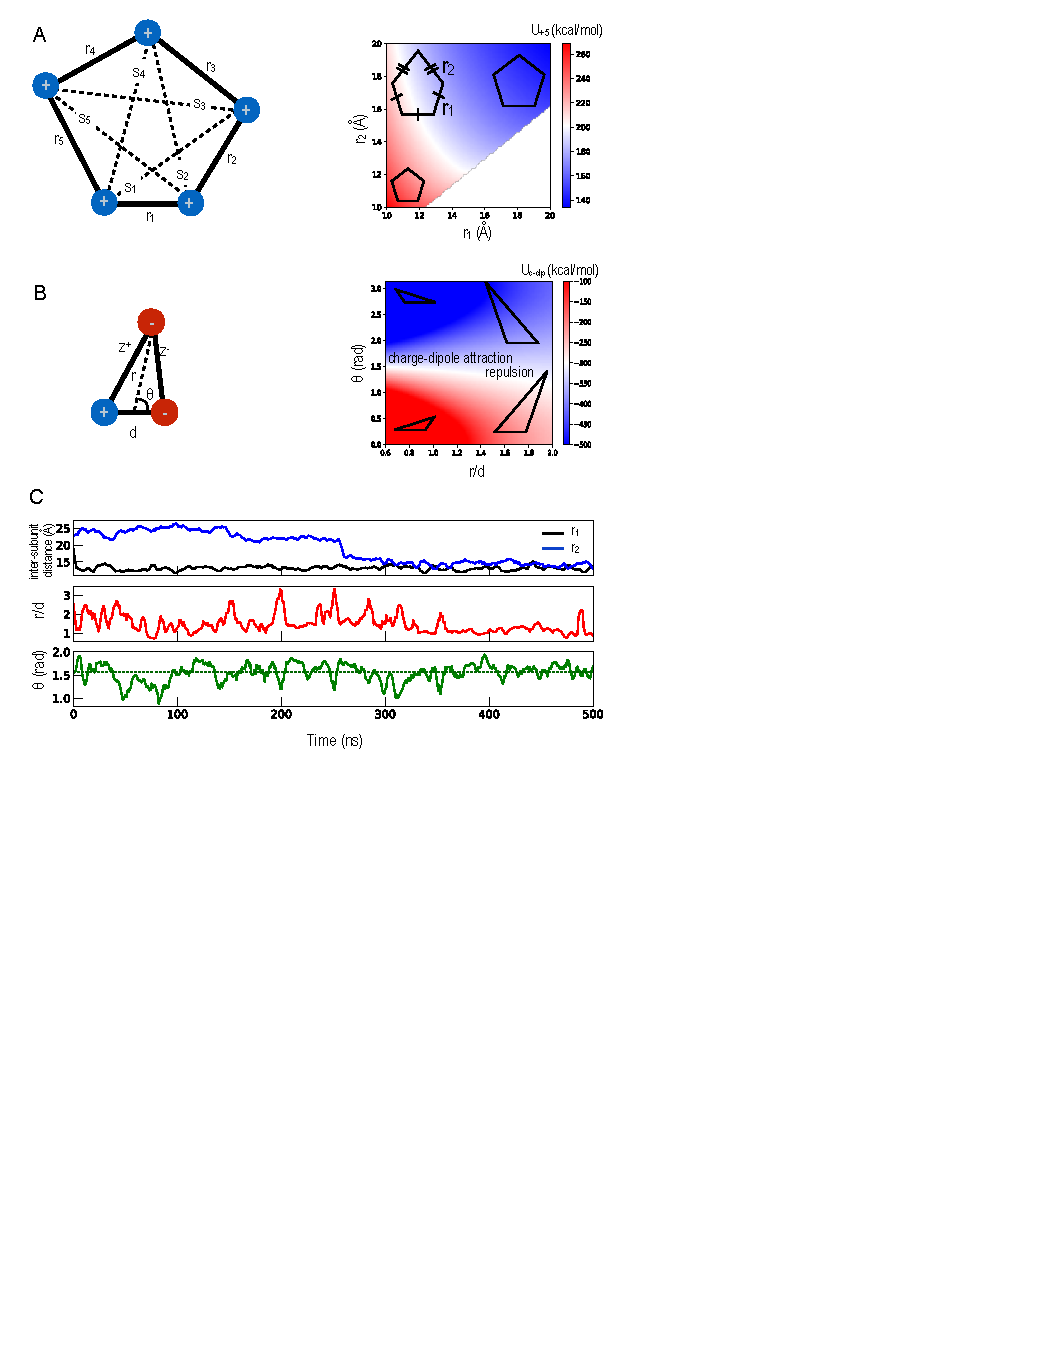
\includegraphics[width = 0.8\textwidth]{figures_2/cartoon_energy.pdf}
\end{center}
\caption{(A) Adjacent and diagonal distances for the pentagonal Interfacial Band used to calculate averages for Eq. \ref{eq:pentamer}, and the associated electrostatic energy for the special case of a pentagon in which three sides are identical and two adjacent sides are also identical, but may differ from the other three.  This special case is similar to that observed for the symmetrization step in Figure 2.  (B) Definition of terms for the charge-dipole interaction that is formed by three residues in the \triad, as well as associated energy. At around $\theta = \pi/2$, the potential energy shifts from decreasing with increasing distance (repulsive) to increasing with increasing distance (attractive).  C) Trajectory for defined angles and distances for the K315 replica explored in Figure 2; curves shown here are smoothed much less than in Figure 2 and retain significantly more high frequency noise. }
\label{fig:cartoon_energy}
\end{figure}

\begin{figure}
\begin{center}
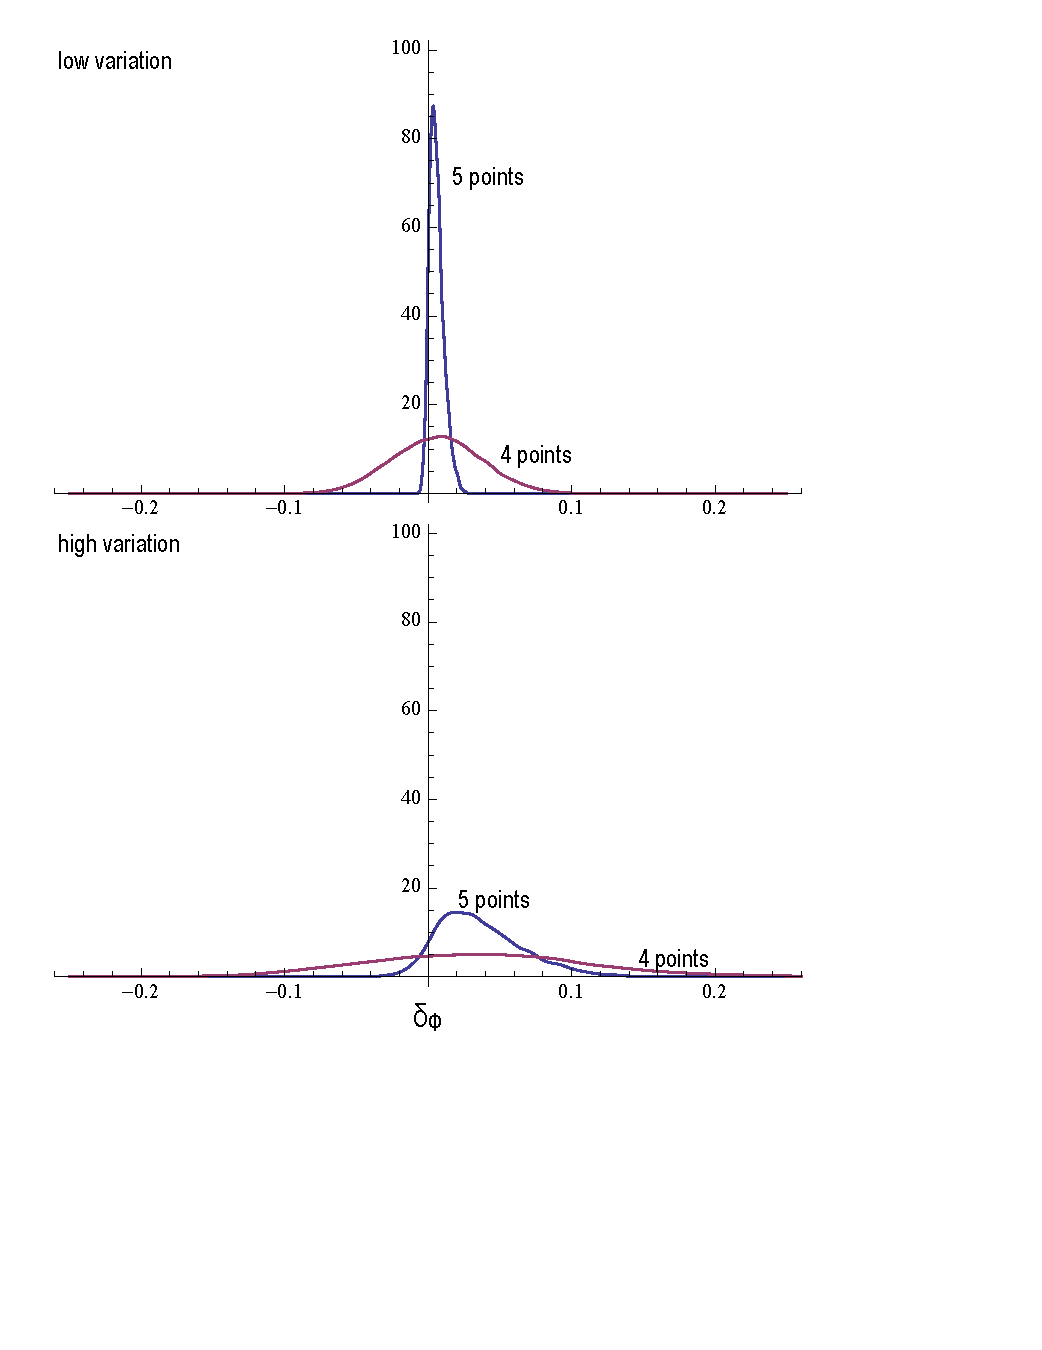
\includegraphics[width = 0.5\textwidth]{figures_2/delta_phi_distribution.pdf}
\end{center}
\caption{Distribution of $\delta_{\phi} \equiv \avgside/\avgdiag - 1/\phi$ for 10,000 trials of five randomly distributed points, with a low or high deviation from a regular pentagonal lattice, as described in Supporting Theory. For the same set of randomly distributed points, $\delta_{\phi}$ was calculated incorporating all five adjacent and diagonal distances into the averages $\avgside$ and $\avgdiag$ (blue line) or only distances involving a 4 point subset (purple line). High deviation is similar to a ``high temperature'' scenario, and the 4 point subset is analogous to the K289M mutant. The energy required to shrink the average side length $\avgside$ will decrease for conformations with low $\delta_{\phi}$, according to Eq. \ref{eq:pentamer}.  }
\label{fig:avgdist}
\end{figure}

\begin{figure}
\begin{texshade}{human_GABAA_aligned_fasta.fasta} 
%2BG9_TM_aligned.fasta.txt is a Fasta file containing an alignment
\shadingmode[charge]{functional}
\shadeallresidues
\nameseq{1}{GABAr:$\alpha_1$}
\nameseq{2}{GABAr:$\alpha_2$}
\nameseq{3}{GABAr:$\alpha_3$}
\nameseq{4}{GABAr:$\alpha_4$}
\nameseq{5}{GABAr:$\alpha_5$}
\nameseq{6}{GABAr:$\alpha_6$}
\nameseq{7}{GABAr:$\beta_1$}
\nameseq{8}{GABAr:$\beta_2$}
\nameseq{9}{GABAr:$\beta_3$}
\nameseq{10}{GABAr:$\gamma_1$}
\nameseq{11}{GABAr:$\gamma_2$}
\nameseq{12}{GABAr:$\gamma_3$}
\residuesperline{29}
\gapchar{-}
%\setdomain{1}{250..339,414..443}
\setends{1}{250..339}
%\setends{1}{414..443}
\feature{ttop}{1}{250..274}{box[Black,White]}{M1}
\feature{ttop}{1}{279..303}{box[Black,White]}{M2}
\feature{ttop}{1}{312..339}{box[Black,White]}{M3}
\feature{ttop}{1}{414..443}{box[Black,White]}{M4}
\feature{ttop}{1}{302..311}{---}{M2-M3 loop}
\feature{bottom}{1}{306..306}{fill:$\uparrow$}{24$^{\prime}$}
\feature{bottom}{1}{302..302}{fill:$\uparrow$}{20$^{\prime}$}
\featurerule{1pt}
%\feature{ttop}{1}{310..311}{fill:\dagger}
\hideconsensus
\end{texshade}
\caption{Alignment of M1, M2, M3 transmembrane helices and M2-M3 loop of  $\alpha$, $\beta$ and $\gamma$ subunits of  human \GABAA  receptors. Residues are colored by charge at pH 7: negatively charged (red) and positively charged (blue). The 24' residue in the M2-M3 loop is a basic residue conserved among all the subunits. The basic residue(K285) in the $\gamma$ subunit and the acidic residue (E270) in $\beta$ subunit which are described as the pore oscillator, forming the charge-dipole interaction are conserved among all the $\beta$ and $\gamma$ subunits.}
\end{figure}

\begin{figure}
\begin{center}
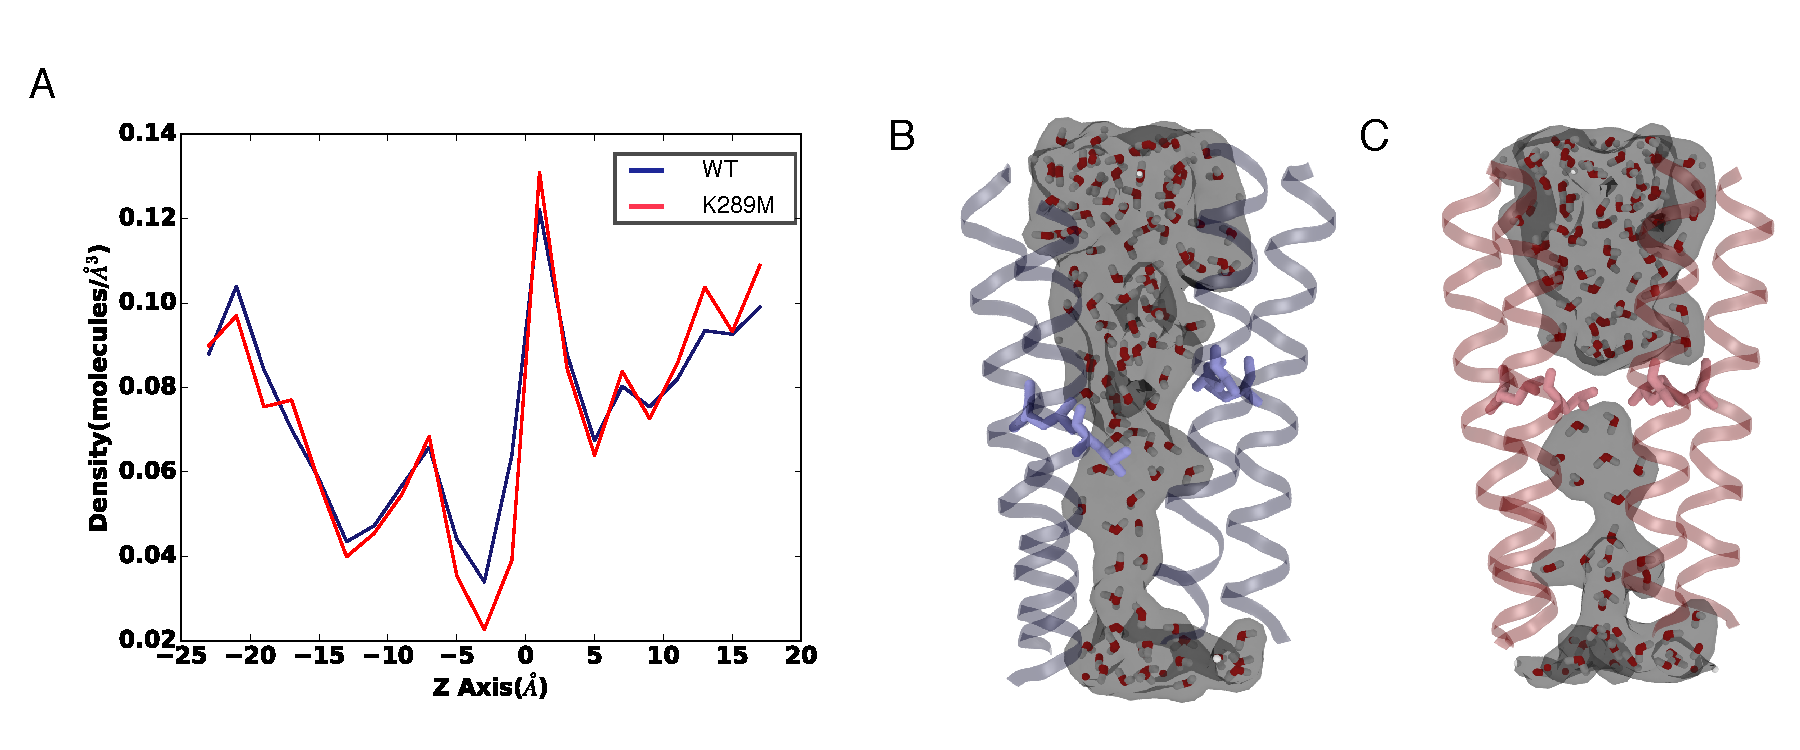
\includegraphics[width = 1\textwidth]{figures_2/water_pore.pdf}
\end{center}
\caption{(A)Number of water molecules along the Z-axis averaged over the frames and replicas. Presence of water in the constriction region of the \WT\ - M2 helices (B) as compared to the temporary dryness due to reduction in pore radii in the  \MT\ - M2 helices(C), at higher temperature. %On an average, nearly zero no. of water molecules are found at the 9' region in the \MT\ system, depicting the stripping of water molecules due to the enclosure of the hydrophobic residues.
}
\label{fig:pore_water}
\end{figure}

\begin{figure}
\begin{center}
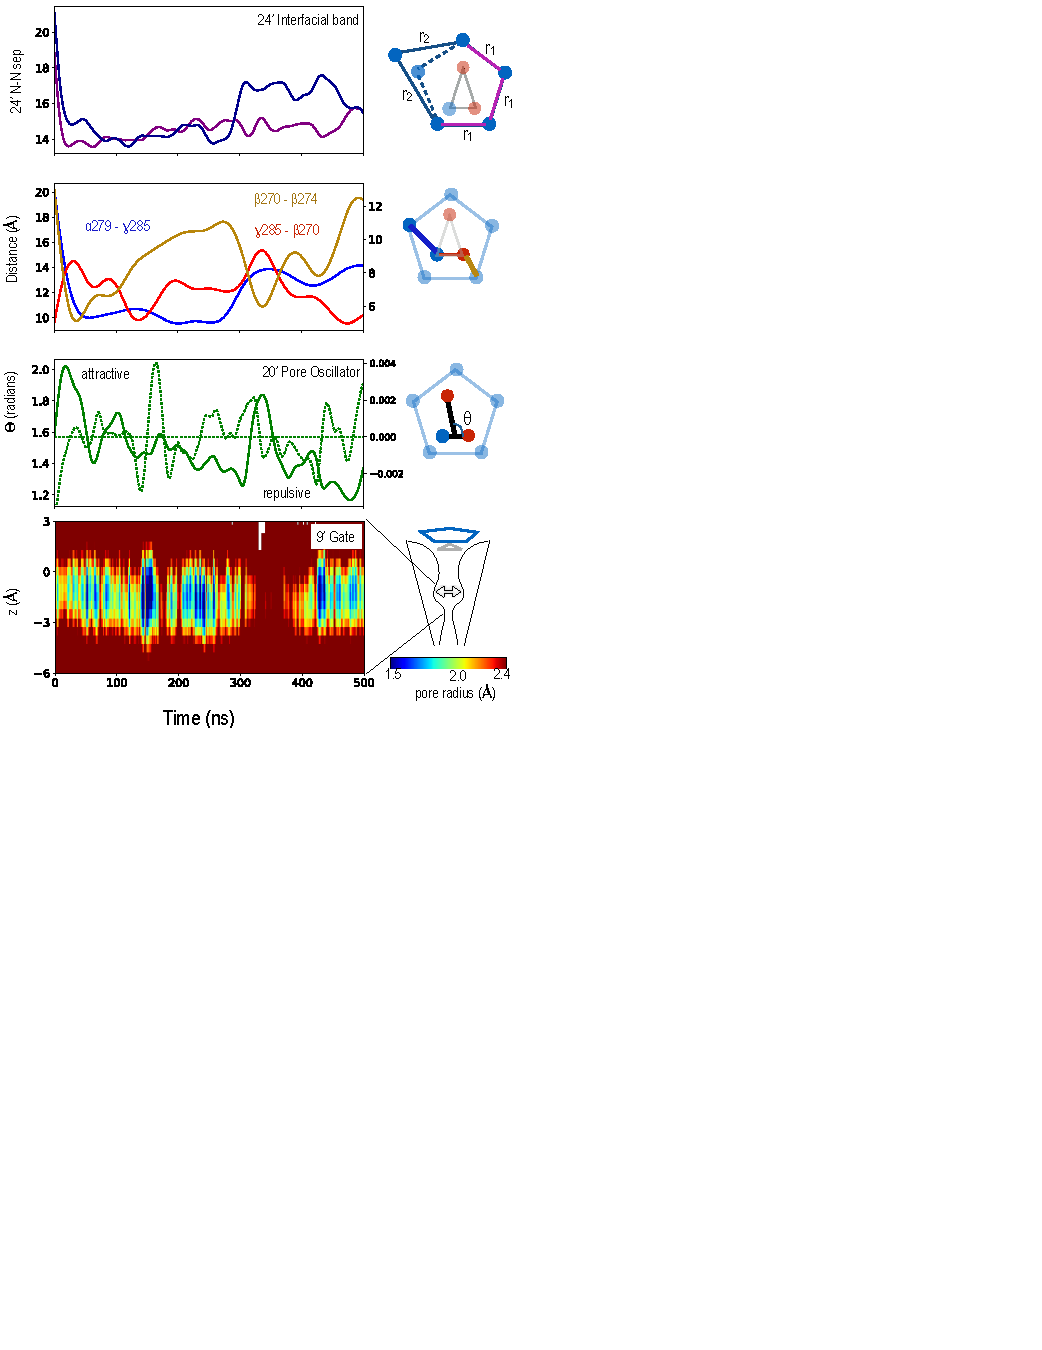
\includegraphics[width = 100mm]{figures_2/pore_opening_events_K300_1.pdf}
\end{center}
\caption{{\bf Evolution of the \fivering and \triad in one replica of the \WT system at 300K.} (A) Flip of one residue ($\alpha$-K279) so the \fivering switches from elongated to regular pentamer, occurs at $\sim$25 ns. (B) The distances between residues $\alpha$K279 -- $\gamma$K285, plotted on y-axis and  $\gamma$K285 -- $\beta$-K270, $\beta$-K270 -- $\beta$-K274, plotted on alternate y-axis, are shown in blue, red and gold respectively. (C) The solid green curve depicts the angle between the charge-dipole arrangement representing the \triad; The Dotted green line represents the pore-opening event as measured by calculating the  first derivative of the minimum pore radii. (D) Pore radius as a function of distance along the pore axis and time.  All curves are smoothed as described in SI Methods.}
\label{fig:K300_1}
\end{figure}

\begin{figure}
\begin{center}
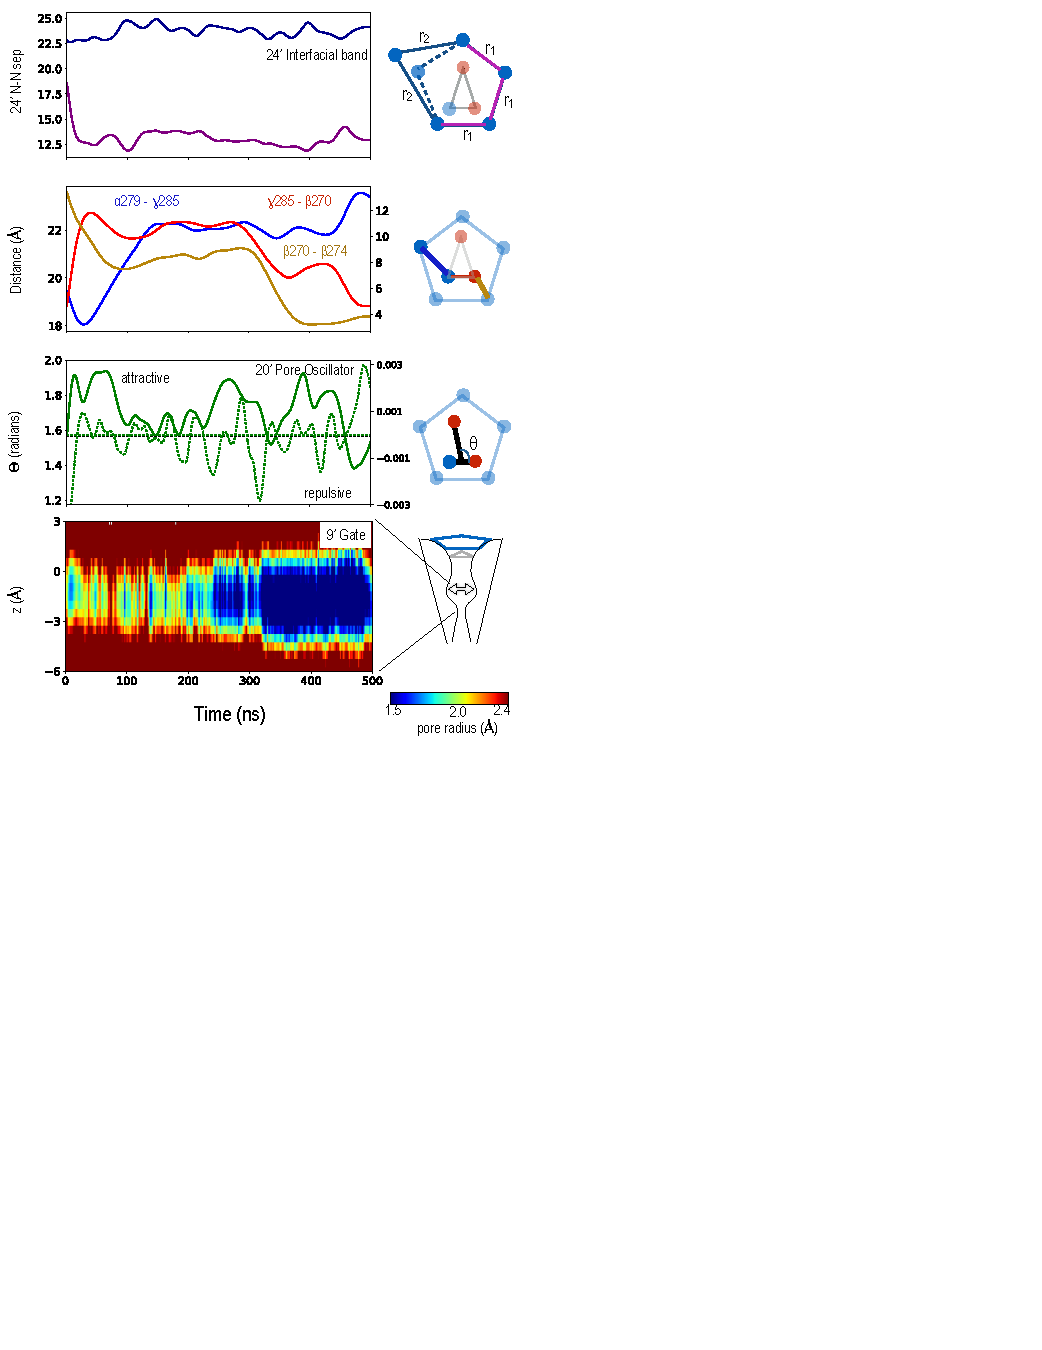
\includegraphics[width = 100mm]{figures_2/pore_opening_events_K300_2.pdf}
\end{center}
\caption{{\bf Evolution of the \fivering and \triad in second replica of the \WT system at 300K.} (A) Flip of one residue ($\alpha$-K279)  does not occur and the \fivering remains in elongated pentamer form. (B) The distances between residues $\alpha$K279 -- $\gamma$K285, plotted on y-axis and  $\gamma$K285 -- $\beta$-K270, $\beta$-K270 -- $\beta$-K274, plotted on alternate y-axis, are shown in blue, red and gold respectively. (C) The solid green curve depicts the angle between the charge-dipole arrangement representing the \triad; The Dotted green line represents the pore-opening event as measured by calculating the  first derivative of the minimum pore radii. (D) Pore radius as a function of distance along the pore axis and time.  All curves are smoothed as described in SI Methods.}
\label{fig:K300_2}
\end{figure}

\begin{figure}
\begin{center}
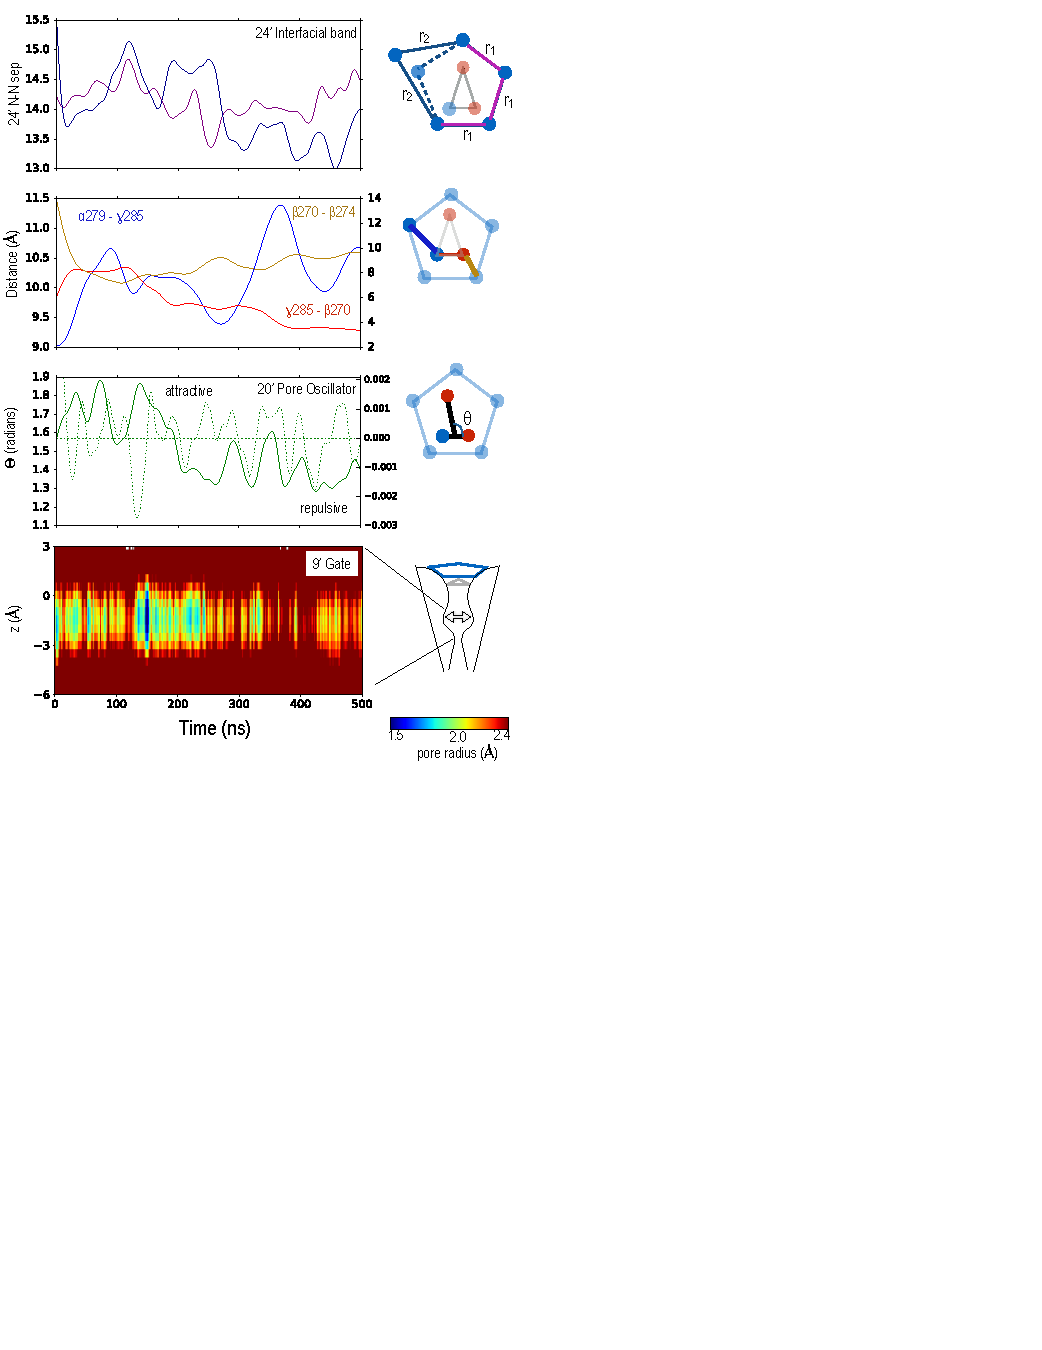
\includegraphics[width = 100mm]{figures_2/pore_opening_events_K315_1.pdf}
\end{center}
\caption{{\bf Evolution of the \fivering and \triad in one replica of the \WT system at 315K.} (A) Residue ($\alpha$-K279) remains flipped from 300K simulations so the \fivering remains in a regular pentamer form. (B) The distances between residues $\alpha$K279 -- $\gamma$K285, plotted on y-axis and  $\gamma$K285 -- $\beta$-K270, $\beta$-K270 -- $\beta$-K274, plotted on alternate y-axis, are shown in blue, red and gold respectively. (C) The solid green curve depicts the angle between the charge-dipole arrangement representing the \triad; The Dotted green line represents the pore-opening event as measured by calculating the  first derivative of the minimum pore radii. (D) Pore radius as a function of distance along the pore axis and time.  All curves are smoothed as described in SI Methods.}
\end{figure}


\begin{figure}
\begin{center}
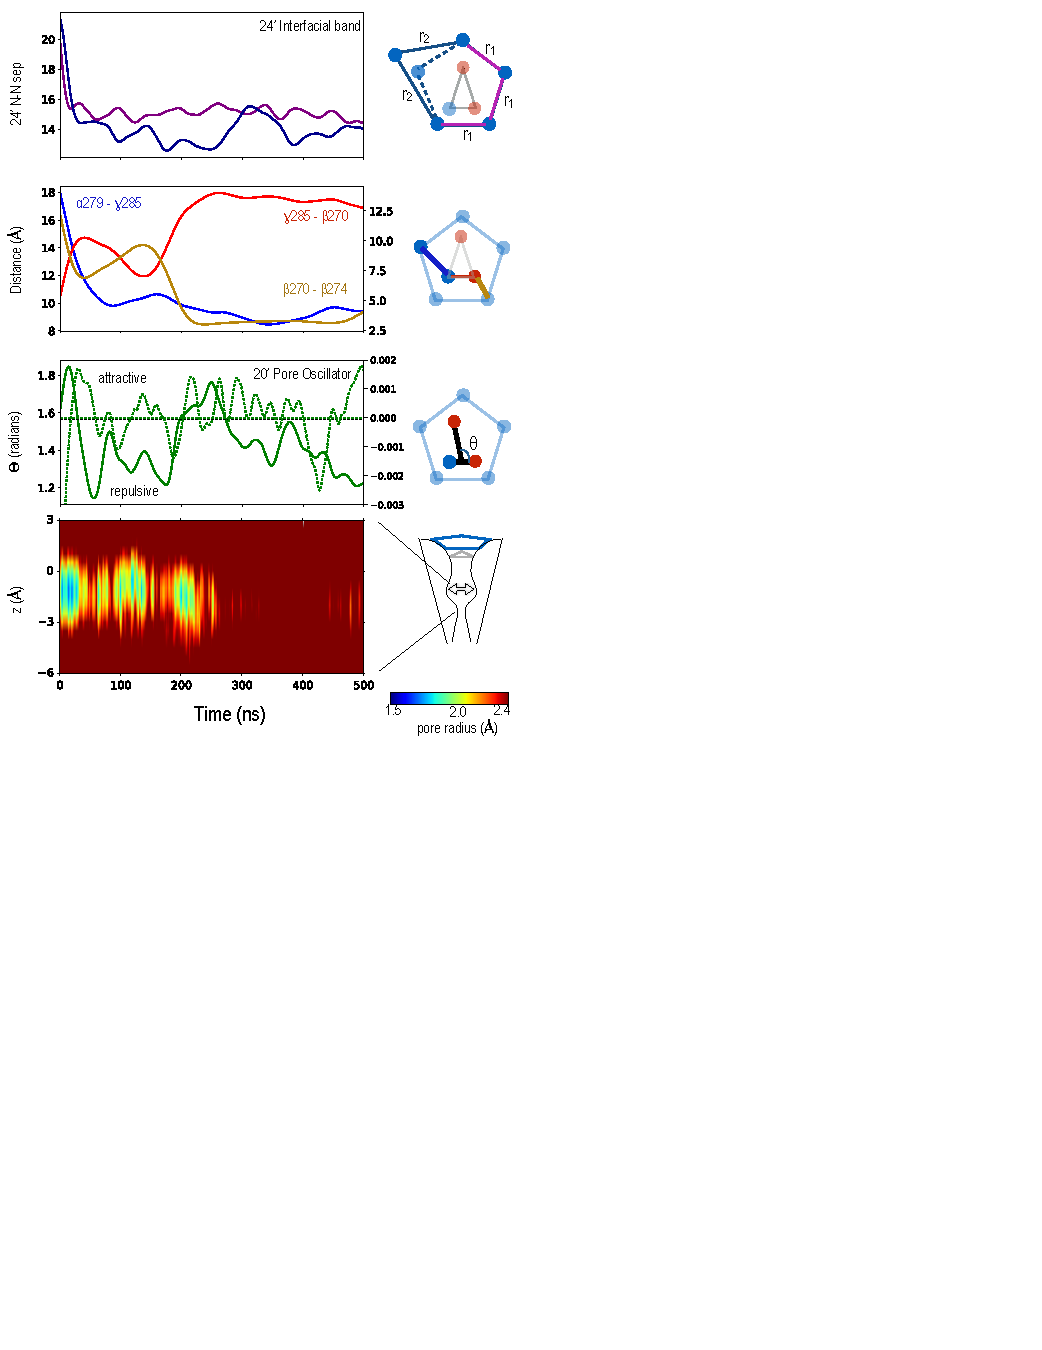
\includegraphics[width = 100mm]{figures_2/pore_opening_events_M300_1.pdf}
\end{center}
\caption{{\bf Evolution of the \fivering and \triad in one replica of the \MT system at 300K.} (A)  Flip of one residue ($\alpha$-K279) so the \fivering switches from elongated to regular pentamer, occurs at $\sim$25 ns. (B) The distances between residues $\alpha$K279 -- $\gamma$K285, plotted on y-axis and  $\gamma$K285 -- $\beta$-K270, $\beta$-K270 -- $\beta$-K274, plotted on alternate y-axis, are shown in blue, red and gold respectively. (C) The solid green curve depicts the angle between the charge-dipole arrangement representing the \triad; The Dotted green line represents the pore-opening event as measured by calculating the  first derivative of the minimum pore radii. (D) Pore radius as a function of distance along the pore axis and time.  All curves are smoothed as described in SI Methods.}
\label{fig:K315_1}
\end{figure}


\begin{figure}
\begin{center}
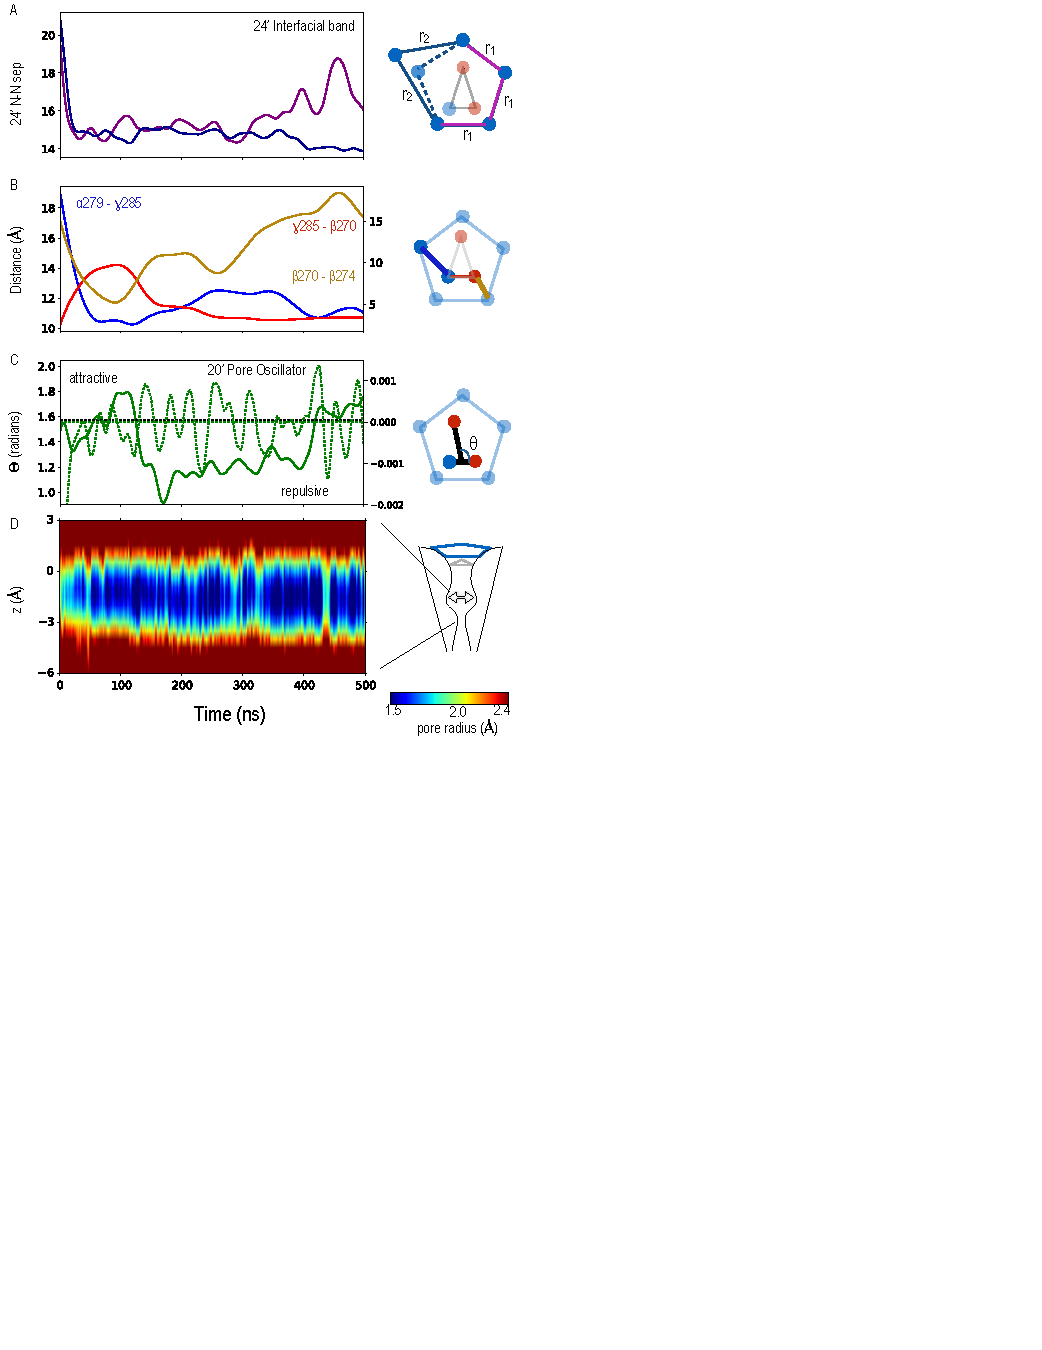
\includegraphics[width = 100mm]{figures_2/pore_opening_events_M300_2.pdf}
\end{center}
\caption{{\bf Evolution of the \fivering and \triad in second replica of the \MT system at 300K.} (A)  Flip of one residue ($\alpha$-K279) so the \fivering switches from elongated to regular pentamer, occurs at $\sim$25 ns. (B) The distances between residues $\alpha$K279 -- $\gamma$K285, plotted on y-axis and  $\gamma$K285 -- $\beta$-K270, $\beta$-K270 -- $\beta$-K274, plotted on alternate y-axis, are shown in blue, red and gold respectively. (C) The solid green curve depicts the angle between the charge-dipole arrangement representing the \triad; The Dotted green line represents the pore-opening event as measured by calculating the  first derivative of the minimum pore radii. (D) Pore radius as a function of distance along the pore axis and time.  All curves are smoothed as described in SI Methods.}
\label{fig:M300_2}
\end{figure}

\begin{figure}
\begin{center}
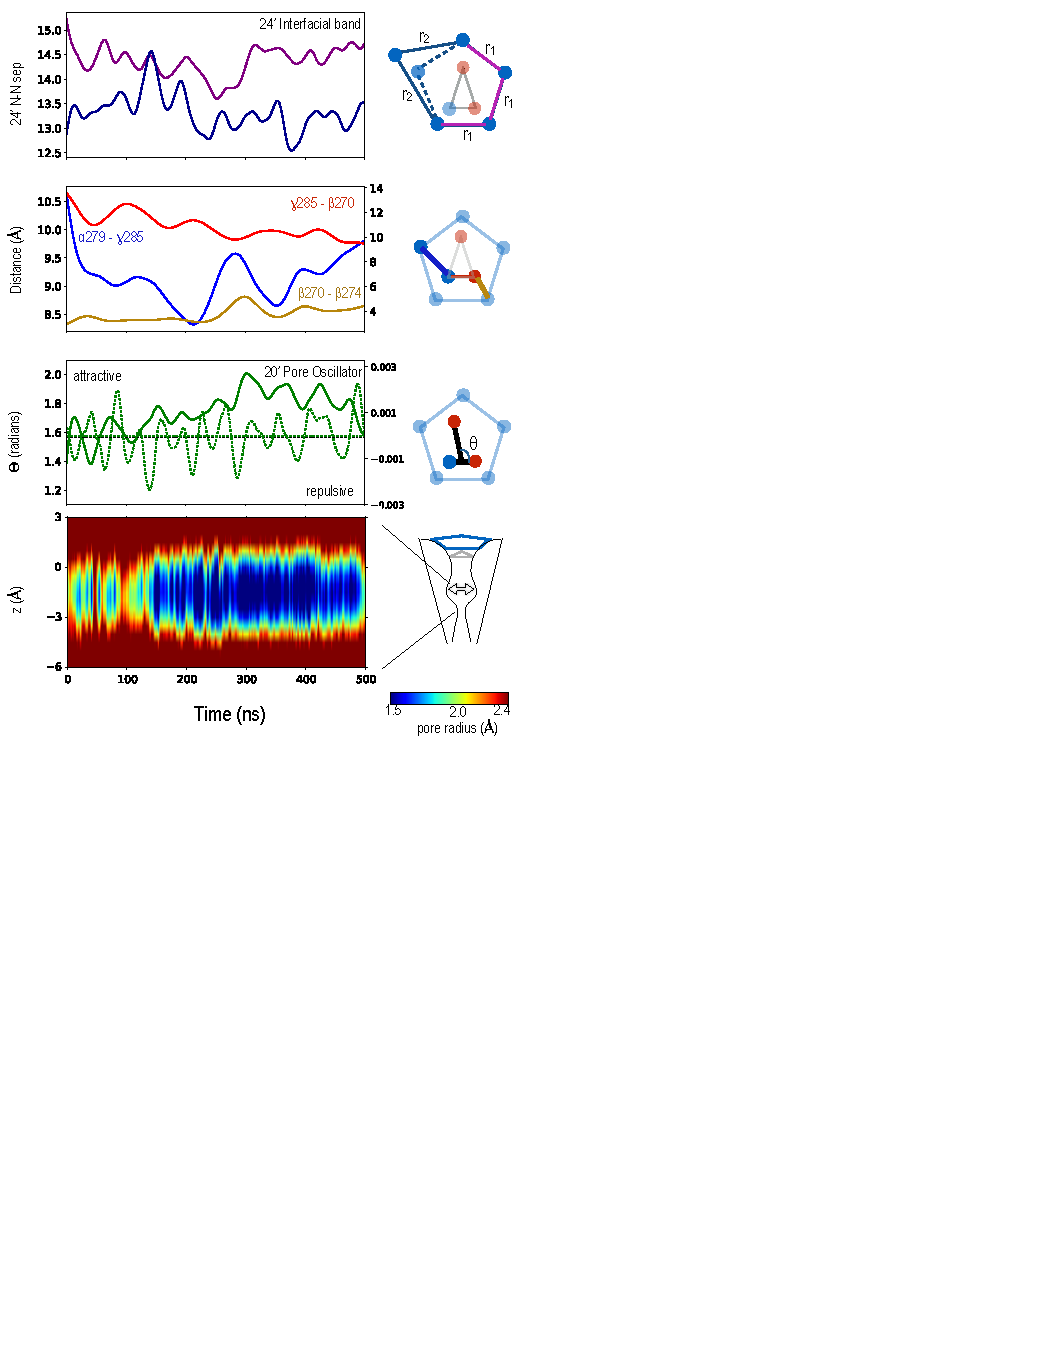
\includegraphics[width = 100mm]{figures_2/pore_opening_events_M315_1.pdf}
\end{center}
\caption{{\bf Evolution of the \fivering and \triad in one replica of the \MT system at 315K.} (A)  Residue ($\alpha$-K279) remains flipped from 300K simulations so the \fivering remains in a regular pentamer form.  (B) The distances between residues $\alpha$K279 -- $\gamma$K285, plotted on y-axis and  $\gamma$K285 -- $\beta$-K270, $\beta$-K270 -- $\beta$-K274, plotted on alternate y-axis, are shown in blue, red and gold respectively. (C) The solid green curve depicts the angle between the charge-dipole arrangement representing the \triad; The Dotted green line represents the pore-opening event as measured by calculating the  first derivative of the minimum pore radii. (D) Pore radius as a function of distance along the pore axis and time.  All curves are smoothed as described in SI Methods.}
\label{fig:M315_1}
\end{figure}

\begin{figure}
\begin{center}
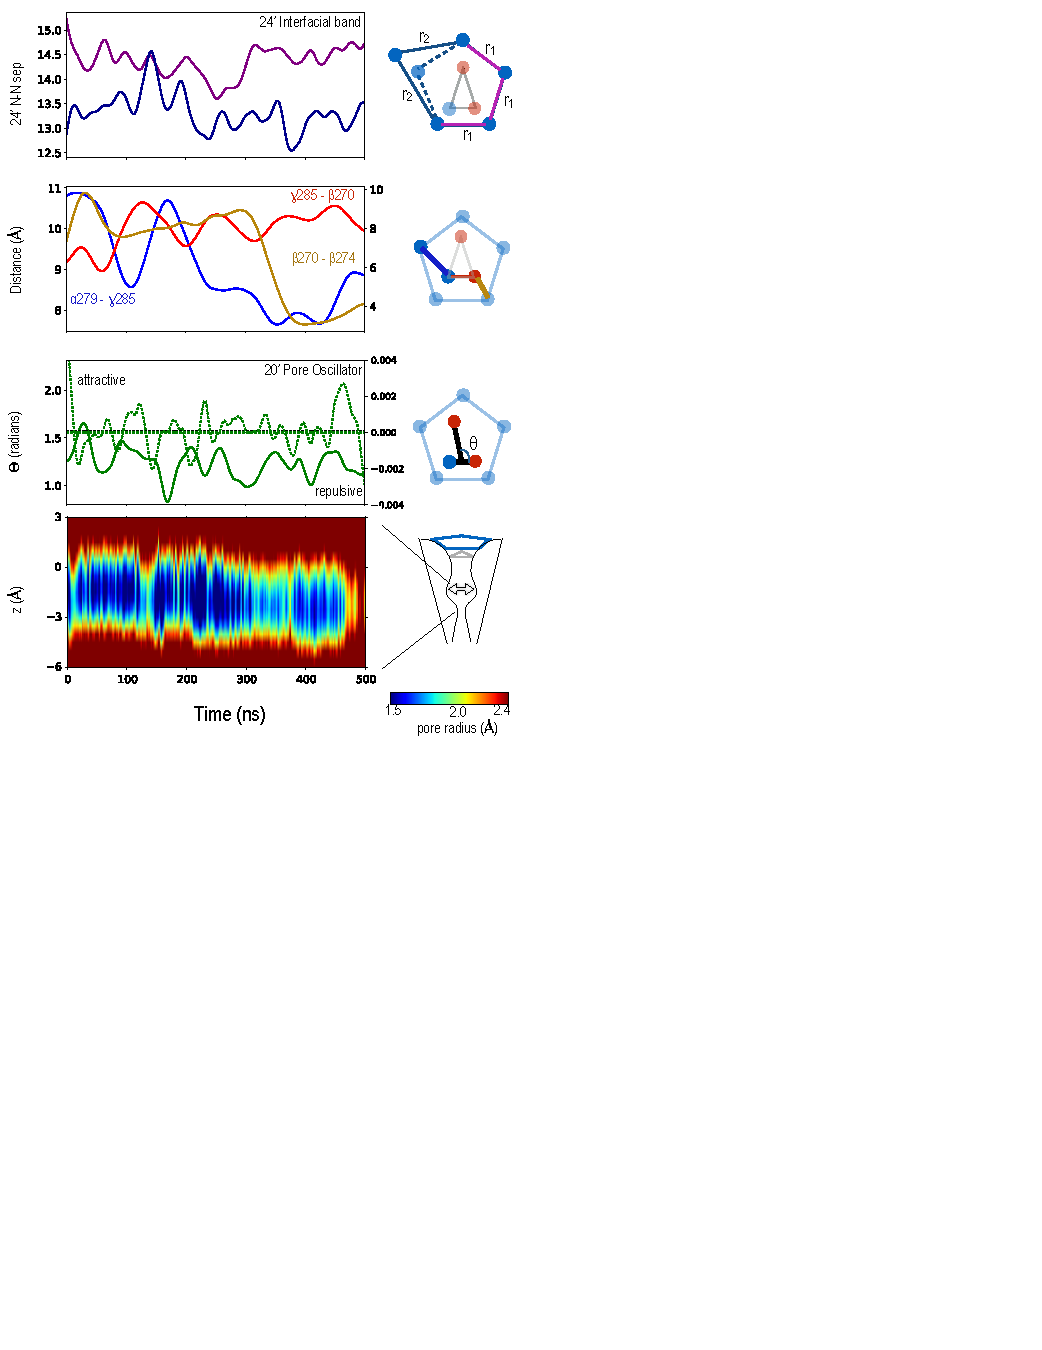
\includegraphics[width = 100mm]{figures_2/pore_opening_events_M315_2.pdf}
\end{center}
\caption{{\bf Evolution of the \fivering and \triad in second replica of the \MT system at 315K.} (A)  Residue ($\alpha$-K279) remains flipped from 300K simulations so the \fivering remains in a regular pentamer form.  (B) The distances between residues $\alpha$K279 -- $\gamma$K285, plotted on y-axis and  $\gamma$K285 -- $\beta$-K270, $\beta$-K270 -- $\beta$-K274, plotted on alternate y-axis, are shown in blue, red and gold respectively. (C) The solid green curve depicts the angle between the charge-dipole arrangement representing the \triad; The Dotted green line represents the pore-opening event as measured by calculating the  first derivative of the minimum pore radii. (D) Pore radius as a function of distance along the pore axis and time.  All curves are smoothed as described in SI Methods.}
\label{fig:M315_2}
\end{figure}

\begin{figure}
\begin{center}
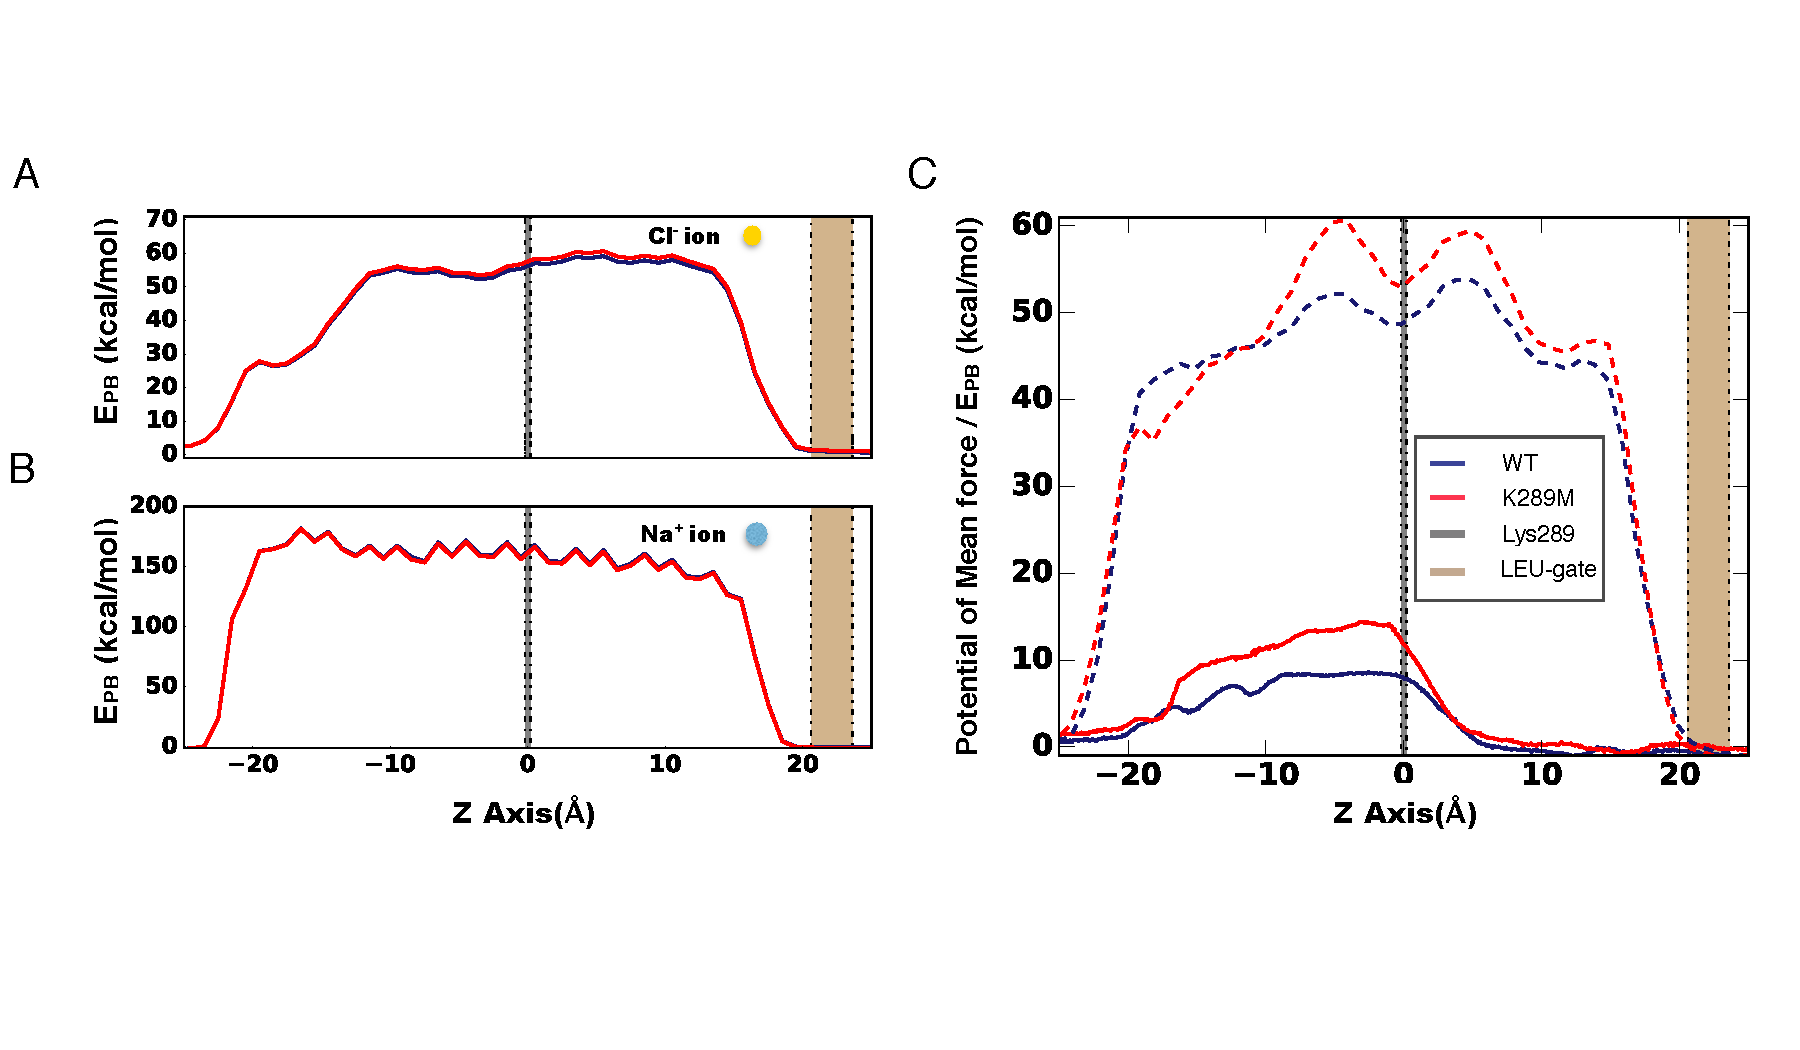
\includegraphics[width = 1\textwidth]{figures_2/sup2_APBS}
\end{center}
\caption{Poisson-Boltzmann profile: (A),(B)Electrostatic environment in the initial configuration of the channel as experienced by a chloride(A) and sodium(B) ion, obtained by performing a Poisson Boltzmann calculation along the TMD. (B)Average of the electrostatic barriers(dotted lines) for the translocation of Chloride ion, between \WT and \MT replicas calculated over the final 50ns of the simulation at 315K, in comparison with the PMF (solid line) calculated using ABF simulations.}
\label{fig:APBS_2}
\end{figure}

%\begin{figure}
%\begin{center}
%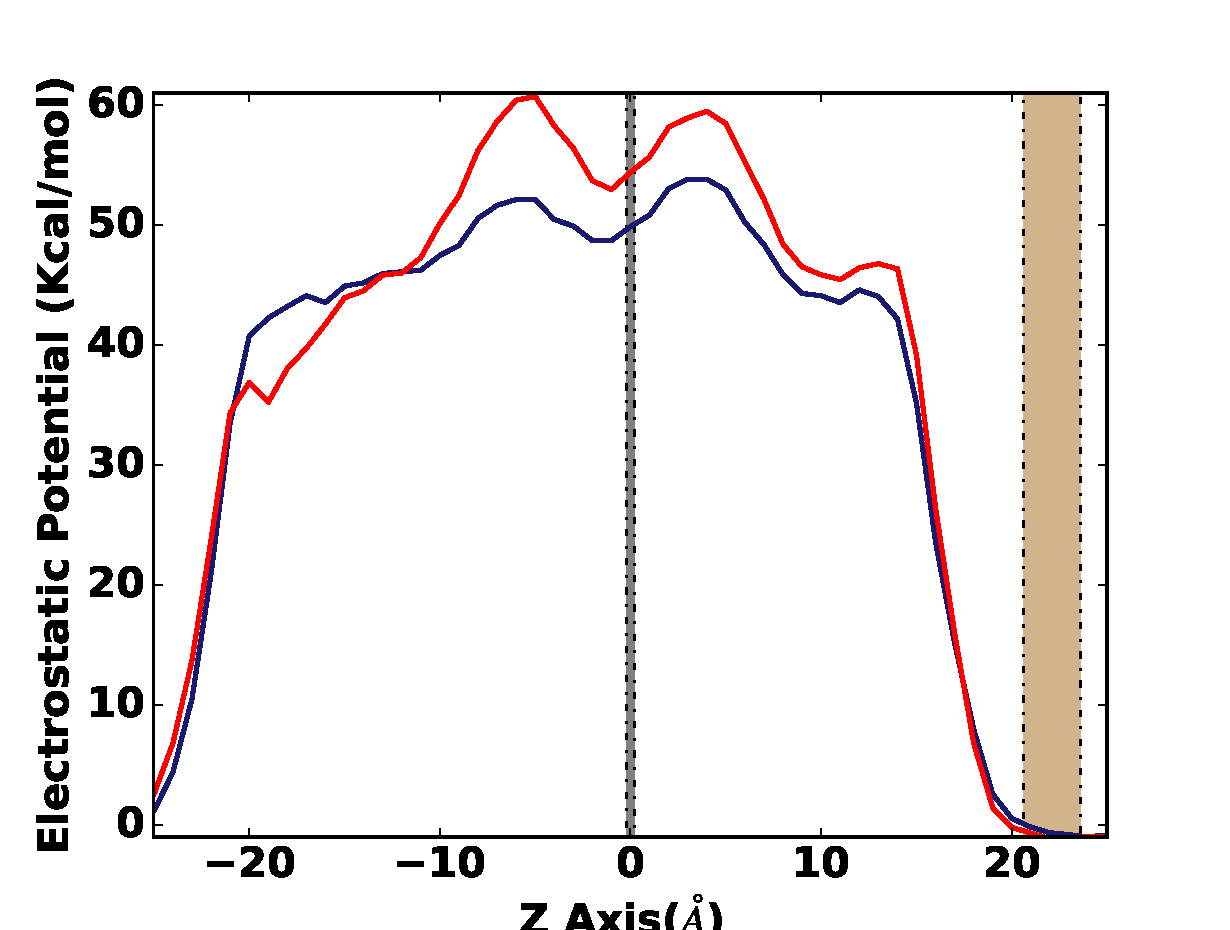
\includegraphics[width = 100mm]{figures/APBS_COMP.pdf}
%\end{center}
%\caption{The Electrostatic potential profiles along the channel pore (for a chloride ion - averaged over 50ns) for the higher  temperature systems. Implicit solvent calculations, performed using APBSmem provided indication about possible barriers in the channel and also the significant difference between the \WT and the \MT.}
%\label{fig:apbs}
%\end{figure}

\begin{figure}
\begin{center}
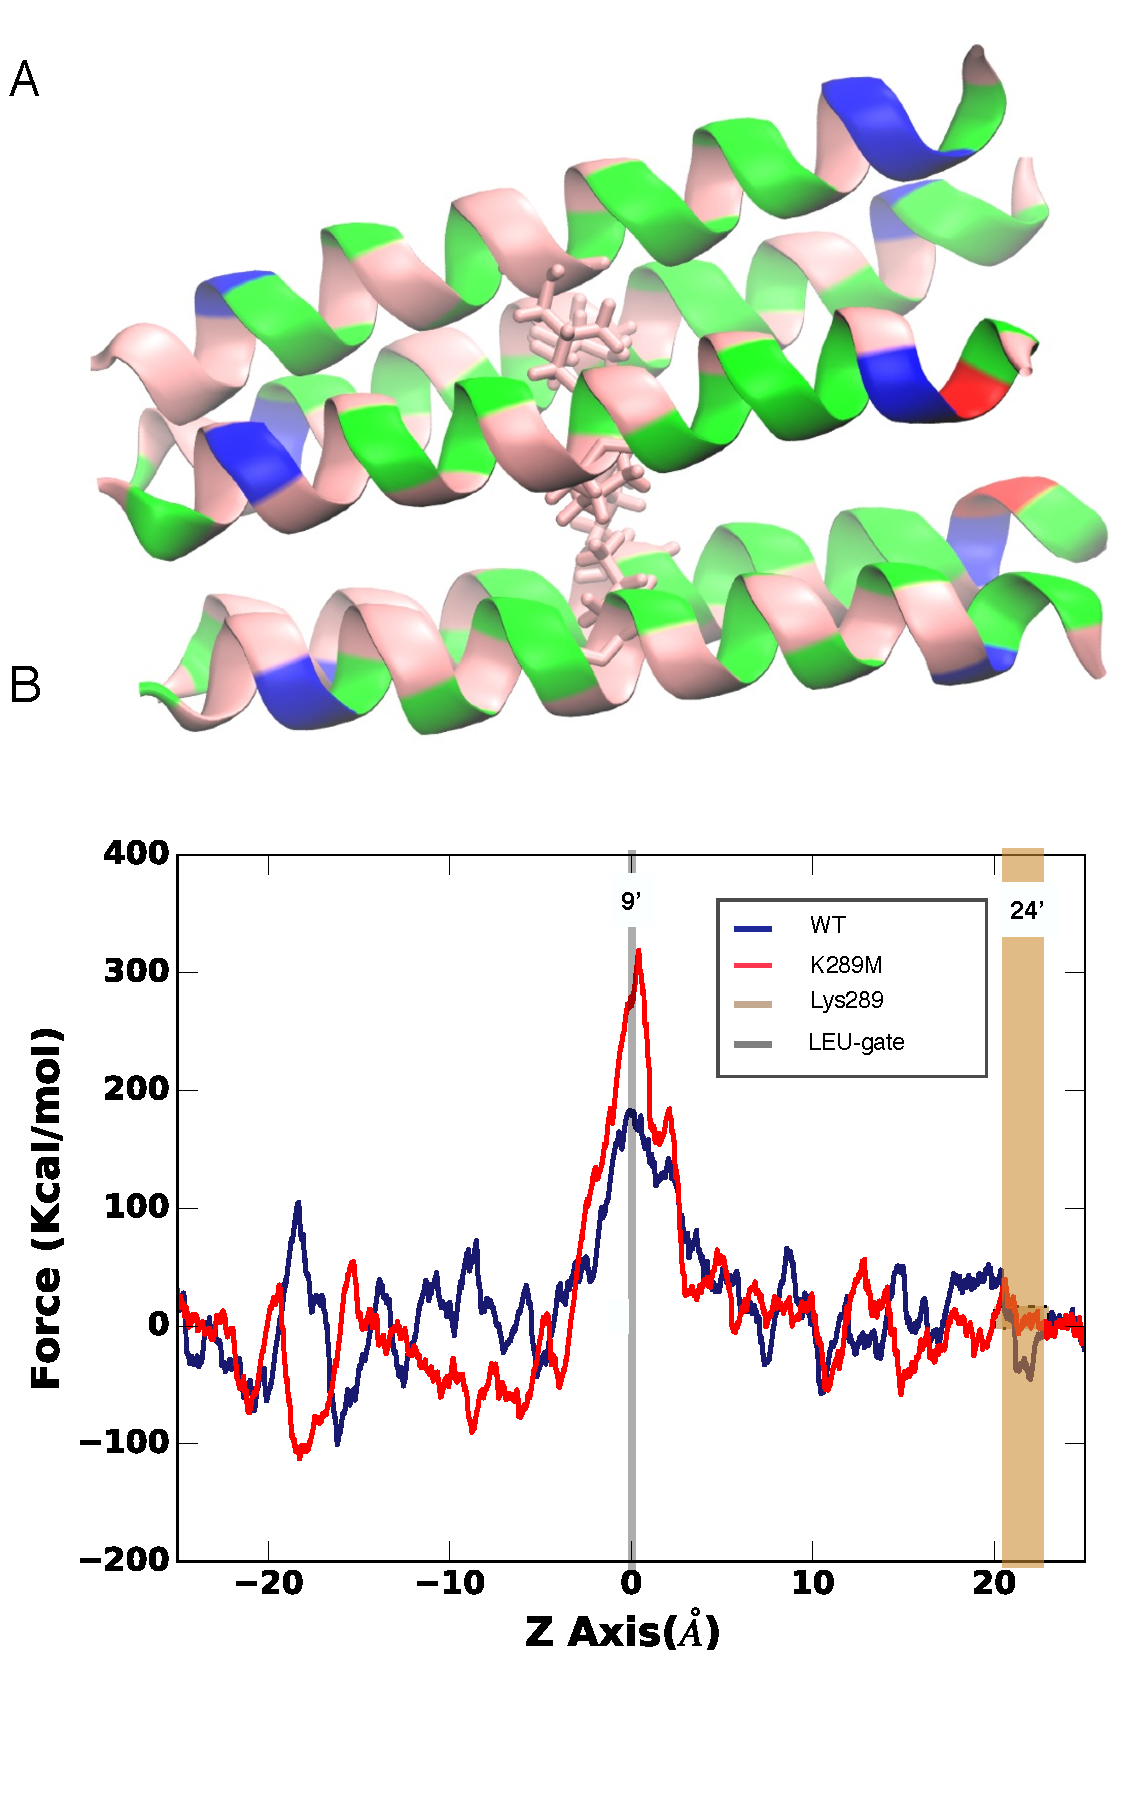
\includegraphics[width = 80mm]{figures_2/sup1_SMD}
\end{center}
\caption{(A) Snap-shot depicting the M2-helices (laid horizontally) showing the minimum constriction region flanked by LEU residues.(B) The force experienced by the ion as a function of position in the channel along the Z axis(TM domain), caluclated by performing SMD on a Chloride passing along the pore of the channel.}
\label{fig:SMD}
\end{figure}

\begin{figure}
\begin{center}
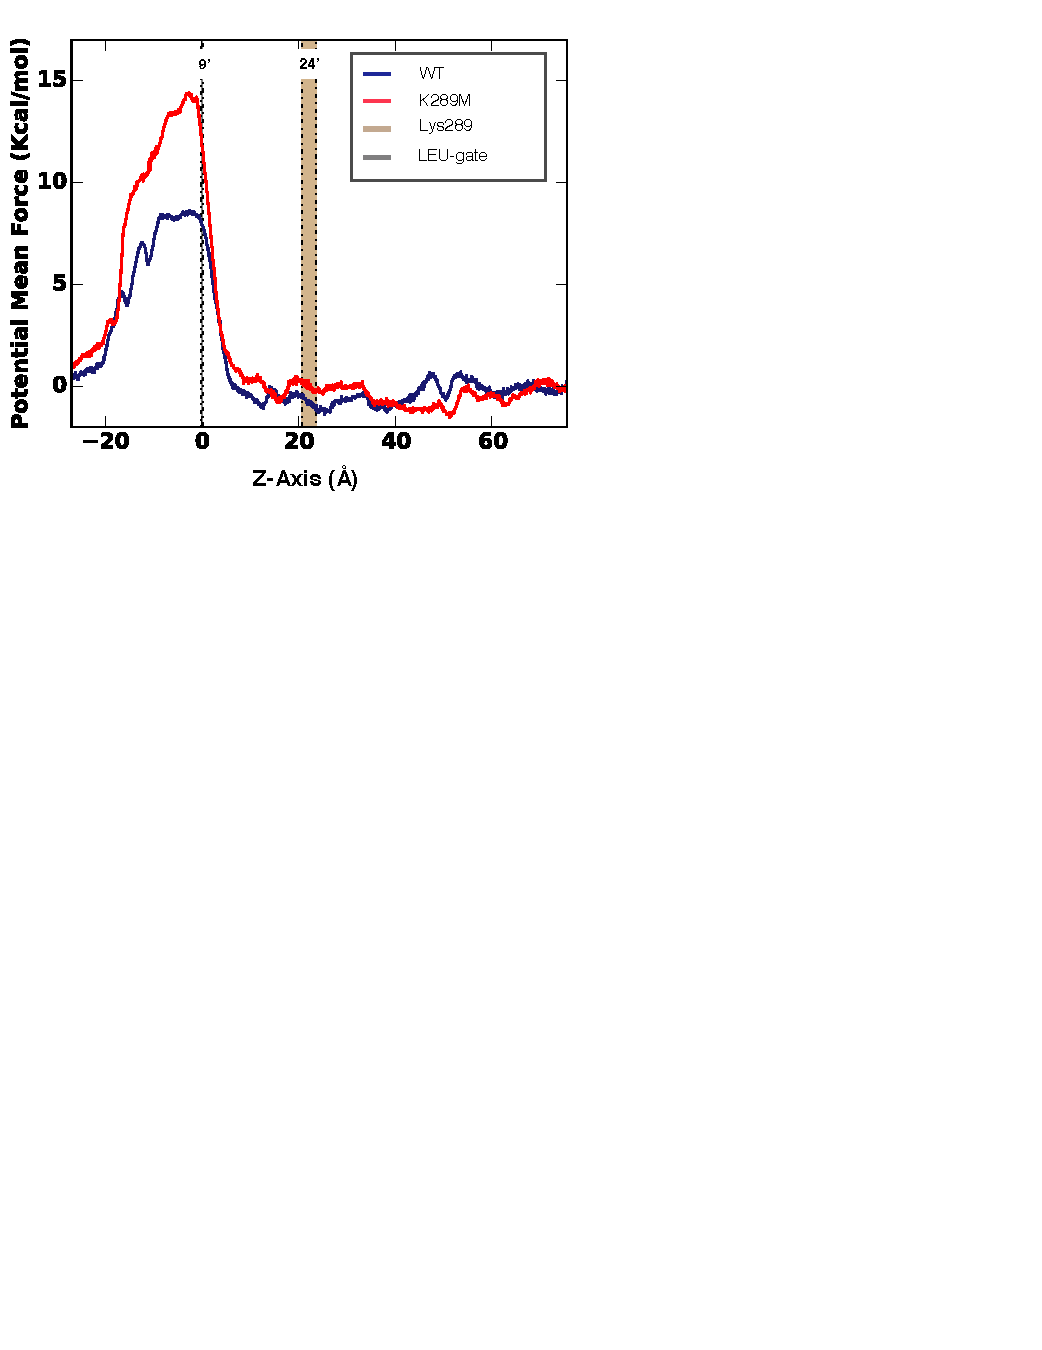
\includegraphics[width = 80mm]{figures_2/pillar_4_ABF_2_sup}
\end{center}
\caption{(A)  Potential of mean force profile of a chloride ion crossing the ion channel, calculated at 315K.}
\label{fig:SMD}
\end{figure}

\begin{figure}
\begin{center}
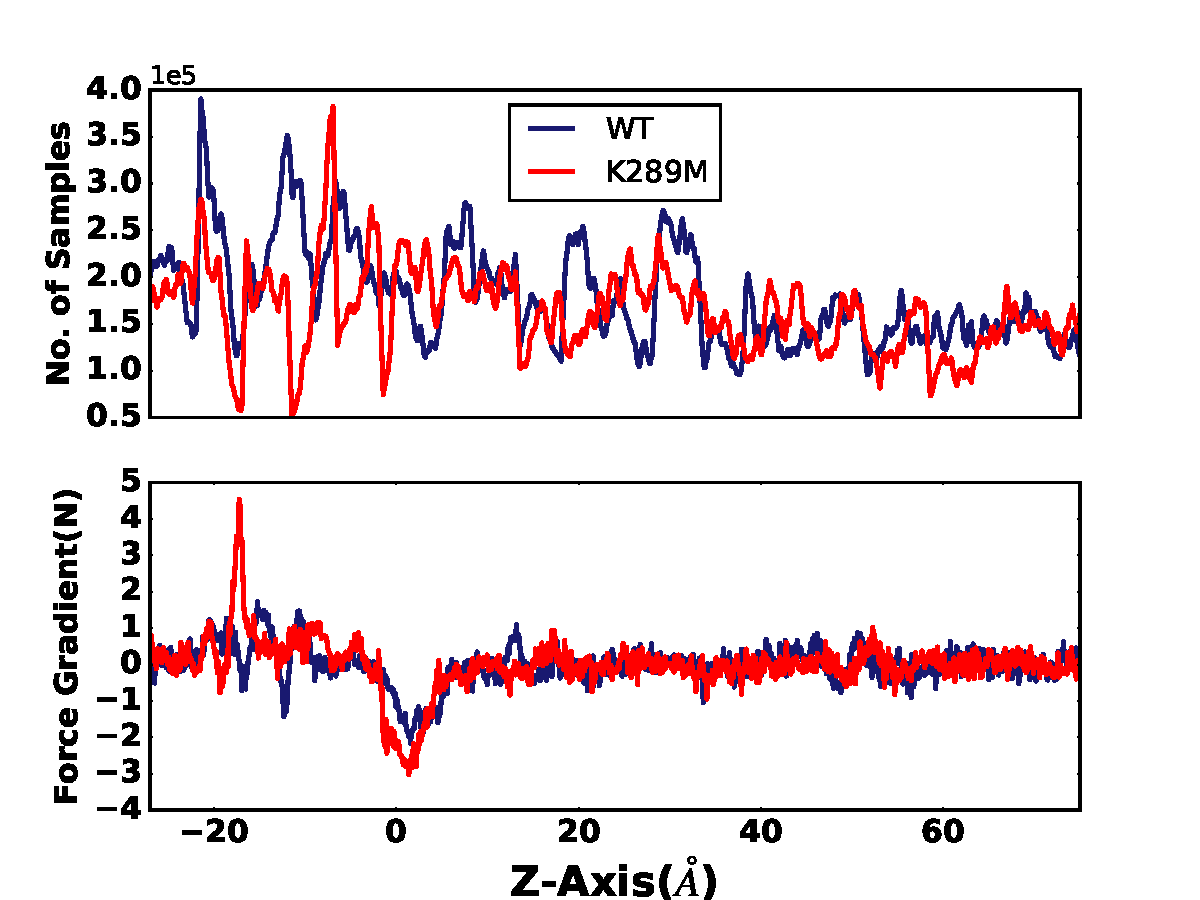
\includegraphics[width = 100mm]{figures_2/Sup_ABF_plots_comp.pdf}
\end{center}
\caption{(A) Number of samples generated in each window of the ABF run. (B) Gradient of the force experienced by the ion in each window of the ABF run. }
\label{fig:ABF_2}
\end{figure}

\clearpage
\bibliographystyle{pnas-new.bst}
\bibliography{GABAa_K289M}
\end{document}